%% -*- TeX-engine: luatex; ispell-language: "russian" -*-

\documentclass[a4paper,12pt]{article}
\usepackage{subcaption}
\usepackage[left=1.5cm,right=2cm,top=1.5cm,bottom=2cm]{geometry}

\usepackage{parskip}
\setlength{\parindent}{0mm}
\setcounter{secnumdepth}{1}

\usepackage{amsmath}

\usepackage{fontspec}
\setmainfont{PT Serif}
\newfontfamily\cyrillicfont[Script=Cyrillic,Ligatures=TeX]{PT Serif}
\setsansfont{PT Sans}
\setmonofont[Ligatures=NoCommon]{PT Mono}
\defaultfontfeatures{Ligatures=TeX}

\usepackage[bold-style=ISO]{unicode-math}
\setmathfont{XITS Math}

\usepackage{microtype}

\usepackage{hyperref}

\usepackage{polyglossia}
\setmainlanguage{russian}
\setotherlanguage{english}

\usepackage{csquotes}

%% for code snippets
\usepackage{minted}
\newminted[pycon]{pycon}{fontsize=\footnotesize}
\newminted[python3]{python3}{fontsize=\footnotesize}
\newminted[bash]{bash}{fontsize=\footnotesize}
\newmintinline[pythoninline]{python3}{fontsize=\footnotesize}
\newmintinline[bashinline]{bash}{fontsize=\footnotesize}

\pagestyle{empty}


\begin{document}
\subsection*{Домашнее задание №7: <<Ядра SVM>>}

\begin{tabular}{@{}lr}
  \textbf{Дедлайн 1} (20 баллов): & 27 апреля, 23:59 \\
  \textbf{Дедлайн 2} (10 баллов): & 4 мая, 23:59
\end{tabular}

Домашнее задание нужно написать на Python и сдать в виде одного файла.
Правило именования файла: \texttt{name\_surname\_7.[py | ipnb]}. Например, если
вас зовут Иван Петров, то имя файла должно быть: \texttt{ivan\_petrov\_7.py} или \texttt{ivan\_petrov\_7.ipnb}.

\makebox[\linewidth]{\hrulefill}

\paragraph{1} Реализуйте Линейный SVM через решение прямой задачи QP для SVM. Рекомендуется воспользоваться пакетом cvxopt \footnote{\url{http://cvxopt.org/userguide/index.html}}. Также обратите внимание на разреженное представление матрицы  \pythoninline{cvxopt.spmatrix}, qp-солвер работает быстрее с разреженными матрицами.
Функция \pythoninline{solvers.qp()} решает задачу следующего вида:


\begin{equation*}
  \begin{cases}
    \frac{1}{2} x^T P x + q^T x \to \min\limits_{x} \\
    Gx \le h \\
    Ax = b
  \end{cases}
\end{equation*}

Необходимо решить следующую задачу оптимизации:

\begin{equation*}
  \begin{cases}
    \frac{1}{2} w^T w + C\sum\limits_{i} \xi_i \to \min\limits_{w, \xi} \\    
    \xi_i \ge 0 \\
    y_i (w^T x_i + w_0) \ge 1 - \xi_i \quad \forall i = 1\dots l
  \end{cases}
\end{equation*}


Сформулируем ее в виде задачи для QP-солвера:
$$x = (w, w_0, \xi)$$\\
$$
\begin{aligned}
  &P = \left[ 
         \begin{array}{c|c}
           I & 0 \\
           \hline
           0 & 0
         \end{array}
       \right]
  \quad
  &q = \left[ 
         \begin{array}{c}
           0 \\
           \hline
           C \cdot 1
         \end{array}
       \right] \\
  &G = \left[
         \begin{array}{c|c|c}
           0 & 0 & -I \\
           \hline
           -y \odot X & -y & -I
         \end{array}
       \right]
  \quad 
  &h = \left[
         \begin{array}{c}
            0 \\
            \hline
            -1
         \end{array}
       \right]
\end{aligned}
$$

Объект $x_i$ является опорным, если в оптимальной точке для задачи линейного SVM неравенство отступов переходит в равенство:
$$y_i (w^T x_i + w_0) = 1 - \xi_i$$

\clearpage
Структура класса приведена ниже:
\begin{python3}
class LinearSVM:
    def __init__(self, C):
        self.C = C
        ...

    def fit(self, X, y):
        ...
        
    def decision_function(self, X):
        ...
        
    def predict(self, X):
        sign(self.decision_function(X))
\end{python3}

\paragraph{2} Реализуйте Ядровой SVM через решение двойственной задачи QP для SVM.

Необходимо решить следующую задачу оптимизации:
\begin{equation*}
  \begin{cases}

    \sum\limits_{i} \alpha_i - \frac{1}{2}\sum\limits_{i}\sum\limits_{j} \alpha_{i}\alpha_{j} y_{i}y_{j} K(x_{i}, x_{j}) \to \max\limits_{\alpha} \\
    0 \le \alpha_i \le C, \quad \forall i = 1, \dots, l \\
    \sum\limits_{i} \alpha_i y_i = 0

  \end{cases}
\end{equation*}

Сформулируем ее в виде задачи для QP-солвера:
$$
\begin{aligned}
    &P = \left[ y_{i}y_{j}K(x_{i}, x_{j}) \right] \quad
    &q = \left[ -1 \right] \\
    &G = \left[ \begin{array}{c} I \\ \hline -I \end{array} \right] \quad \quad
    &h = \left[ \begin{array}{c} C\cdot 1 \\ \hline 0 \end{array} \right] \\
    &A = y^T\quad
    &b = 0
\end{aligned}
$$

Объект $x_i$ является опорным, если $\alpha_i > 0$.

Решение принимается по следующему правилу:
$$a(x) = \text{sign}\left(\sum\limits_{i}\alpha_{i}y_{i}K(x, x_{i}) + w_0\right).$$

Для предсказания необходимо оценить значение $w_0$. Известно, что для любого опорного объекта, который классифицируется безошибочно, верно следующее:
$$y_i = \sum\limits_{j}\alpha_{j}y_{j} K(x_{i}, x_{j}) + w_0,$$
значит для любого такого объекта:

$$w_0 = y_i - \sum\limits_{j}\alpha_{j} y_{j} K(x_{i}, x_{j})$$

В случае наличия ошибок классификации обучающей выборки предлагается усреднять значение $w_0$ по всем опорным векторам:

$$w_0 = \frac{1}{N_\text{SV}}\sum_{n \in \text{SV}} \left(y_i - \sum\limits_{j} \alpha_{j} y_{j} K(x_{i}, x_{j})\right).$$

Интуиция здесь такова, что суммарные ошибки в положительную сторону примерно равны суммарным ошибкам в отрицательную сторону.

Структура класса аналогична:
\begin{python3}
class KernelSVM:
    def __init__(self, C, kernel=None, sigma=1.0, degree=2):
        self.C = C
        ...
    
    def fit(self, X, y):
        ...
    
    def decision_function(self, X):
        ...
        
    def predict(self, X):
        ...
\end{python3}

Параметр конструктора \pythoninline{degree} понадобится при использовании полиномиального ядра, игнорируется другими ядрами. Параметр \pythoninline{sigma} используется для гауссовского ядра. Параметры конструктора соответствуют параметрам стандартного SVM в Scikit-learn \footnote{\url{http://scikit-learn.org/stable/modules/svm.html}}.

\paragraph{3} Реализуйте полиномиальное и гауссовское ядра. Функция должна принимать на вход две матрицы объектов X и возвращать матрицу K.

Например, линейное ядро выглядит следующим образом:
\begin{python3}
import numpy as np

def linear_kernel(X1, X2):
    return np.dot(X1, X2)
\end{python3}

\paragraph{4} Воспользуйтесь визуализатором разделяющей поверхности, приведенным по ссылке\footnote{\url{https://gist.github.com/ktisha/ae995b7b553db26316f9}} или напишите свой с соответствующей сигнатурой.

\begin{python3}
def visualize(clf, X, y):
  ...
\end{python3}


\paragraph{5} Протестируйте следующие алгоритмы на случайных выборках с признаками длины 2 и визуализируйте на плоскости получающиеся решающие правила.
\begin{enumerate}
  \item Линейная разделяющая гиперплоскость обученная линейным SVM и обученная ядровым SVM с линейным ядром
  \item Квадратичная разделяющая гиперплоскость (ядровой SVM с полиномиальным ядром степени 2)
  \item Radial basis function SVM (ядровой SVM с гауссовским ядром)
\end{enumerate}

Для генерации случайных наборов данных можно воспользоваться SciKit-Learn \footnote{\url{http://scikit-learn.org/stable/datasets/\#sample-generators}}

\paragraph{6} Поварьируйте параметры классификатора. Что можно сказать про влияние параметров на классификацию?\\


Пример полученной визуализации для RBF ядра с разными значениями \sigma

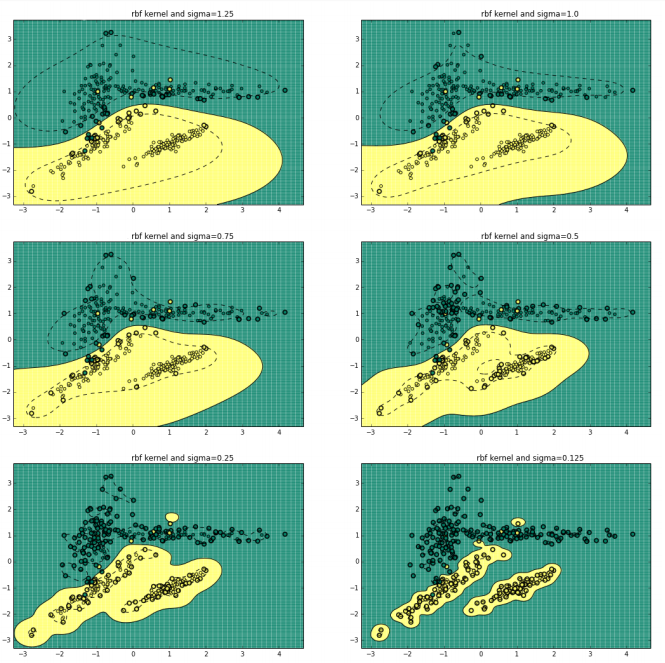
\includegraphics[width=\textwidth, keepaspectratio]{images/visualization}

\end{document}
